\documentclass[a4paper,oneside,12pt]{report}
% Package yang diperlukan
\usepackage{graphicx}      % Untuk memasukkan gambar
\usepackage{titling}       % Untuk kustomisasi halaman judul
\usepackage{geometry}      % Untuk mengatur margin halaman
\usepackage{listings}      % Untuk menampilkan blok kode
\usepackage{xcolor}        % Untuk menggunakan warna
\usepackage{float}         % Untuk kontrol penempatan float (seperti gambar)
\usepackage{hyperref}      % Untuk membuat hyperlink (URL, referensi)
\usepackage{indentfirst}   % Untuk memberi indentasi pada paragraf pertama setiap seksi
\usepackage{url}           % Untuk format URL
\usepackage{fancyhdr}      % Untuk kustomisasi header dan footer
\usepackage{tocloft}       % Untuk kustomisasi Daftar Isi
\usepackage{bookmark}      % Untuk manajemen bookmark PDF yang lebih baik

%======================================================================
% PENGATURAN GEOMETRI HALAMAN
%======================================================================
% Margin umum untuk isi laporan
\geometry{left=3cm, right=2.5cm, top=2cm, bottom=2.5cm}
\sloppy

%======================================================================
% PENGATURAN WARNA UNTUK BLOK KODE
%======================================================================
\definecolor{codegreen}{rgb}{0,0.6,0}
\definecolor{codegray}{rgb}{0.5,0.5,0.5}
\definecolor{codepurple}{rgb}{0.58,0,0.82}
\definecolor{backcolour}{rgb}{0.95,0.95,0.92}
\definecolor{darkblue}{rgb}{0,0,0.6}

%======================================================================
% PENGATURAN BLOK KODE (LISTINGS)
%======================================================================
% Gaya umum untuk semua blok kode
\lstdefinestyle{commonstyle}{
    backgroundcolor=\color{backcolour}, 
    breakatwhitespace=false, 
    breaklines=true, 
    captionpos=b, 
    keepspaces=true,
    numbers=left, 
    numbersep=5pt, 
    showspaces=false, 
    showstringspaces=false,
    showtabs=false, 
    tabsize=2, 
    frame=single,
    basicstyle=\ttfamily\footnotesize,
    numberstyle=\tiny\color{codegray},
    columns=flexible,
    postbreak=\mbox{\textcolor{red}{$\hookrightarrow$}\space},
    breakindent=0pt,
    breakautoindent=false
}

% Gaya khusus untuk HTML
\lstdefinestyle{htmlstyle}{
    style=commonstyle,
    language=HTML,
    commentstyle=\color{codegreen},
    keywordstyle=\color{codepurple},
    stringstyle=\color{codegreen},
    basicstyle=\ttfamily\scriptsize
}

% Gaya khusus untuk CSS
\lstdefinestyle{cssstyle}{
    style=commonstyle,
    commentstyle=\color{codegreen},
    keywordstyle=\color{darkblue},
    stringstyle=\color{codepurple},
    emph={color, background, font, margin, padding, border, display, position, width, height},
    emphstyle=\color{darkblue},
    basicstyle=\ttfamily\scriptsize
}

% Gaya khusus untuk Python
\lstdefinestyle{pythonstyle}{
    style=commonstyle,
    language=Python,
    commentstyle=\color{codegreen},
    keywordstyle=\color{darkblue},
    stringstyle=\color{codepurple},
    emph={import,from,class,def,for,while,if,else,elif,try,except,finally},
    emphstyle=\color{darkblue}
}

% Gaya khusus untuk SQL
\lstdefinestyle{sqlstyle}{
    style=commonstyle,
    language=SQL,
    commentstyle=\color{codegreen},
    keywordstyle=\color{darkblue},
    stringstyle=\color{codepurple},
    emph={SELECT,FROM,WHERE,INSERT,UPDATE,DELETE,CREATE,DROP},
    emphstyle=\color{darkblue}
}

% Gaya khusus untuk JavaScript
\lstdefinestyle{javascriptstyle}{
    style=commonstyle,
    language=JavaScript,
    commentstyle=\color{codegreen},
    keywordstyle=\color{darkblue},
    stringstyle=\color{codepurple},
    emph={function,var,let,const,return,if,for,while,do,else,switch,case},
    emphstyle=\color{darkblue}
}

%======================================================================
% PENGATURAN LAIN-LAIN
%======================================================================
% Perintah kustom untuk bingkai gambar
\newcommand{\customfbox}[1]{%
  \setlength{\fboxsep}{0pt}%
  \setlength{\fboxrule}{0.5pt}%
  \fcolorbox{black}{white}{#1}%
}

% Mengganti nama default "Figure" menjadi "Gambar"
\renewcommand{\figurename}{Gambar}
\renewcommand{\thefigure}{\arabic{figure}}

% Pengaturan Hyperlink
\hypersetup{
    colorlinks=true, 
    linkcolor=black, 
    filecolor=black, 
    urlcolor=black,
    citecolor=black,
    pdftitle={Laporan Praktikum}, 
    pdfpagemode=FullScreen, 
    breaklinks=true
}

% Pengaturan Header & Footer (nomor halaman di tengah bawah)
\pagestyle{fancy}
\fancyhf{}
\fancyfoot[C]{\thepage}
\renewcommand{\headrulewidth}{0pt}

\fancypagestyle{plain}{
    \fancyhf{}
    \fancyfoot[C]{\thepage}
    \renewcommand{\headrulewidth}{0pt}
}

%======================================================================
% PENGATURAN STRUKTUR BAB DAN DAFTAR ISI
%======================================================================
\renewcommand{\contentsname}{Daftar Isi}
\renewcommand{\bibname}{Daftar Pustaka}

% Menghilangkan nomor bab tetapi mempertahankan penomoran seksi
\renewcommand{\thechapter}{}
\renewcommand{\chaptername}{}

% Format penomoran seksi menjadi [nomor bab].[nomor seksi]
\renewcommand{\thesection}{\arabic{chapter}.\arabic{section}}
\renewcommand{\thesubsection}{\thesection.\arabic{subsection}}

\setcounter{secnumdepth}{3}
\setcounter{tocdepth}{3}

% Format Daftar Isi (TOC)
\renewcommand{\cftchapdotsep}{\cftdotsep}
\renewcommand{\cftchapleader}{\cftdotfill{\cftchapdotsep}}
\setlength{\cftchapindent}{0em}
\setlength{\cftsecindent}{2em}
\setlength{\cftsubsecindent}{4em}
\setlength{\cftchapnumwidth}{0em}
\setlength{\cftsecnumwidth}{2.5em}
\setlength{\cftsubsecnumwidth}{3.2em}
\renewcommand{\cftchappresnum}{}
\renewcommand{\cftchapaftersnum}{}

% Perintah kustom untuk membuat judul bab di TOC menjadi tebal
\newcommand{\tocboldsection}[1]{%
  \protect\renewcommand{\protect\cftchapfont}{\protect\bfseries}%
  #1%
  \protect\renewcommand{\protect\cftchapfont}{}%
}

%======================================================================
% AWAL DOKUMEN
%======================================================================
\begin{document}

% Halaman Judul
\newgeometry{left=3cm, right=2.5cm, top=2.5cm, bottom=3cm}
\begin{titlingpage}
\begin{center}
\vspace*{0.5cm}
{\large \textbf{\MakeUppercase{Laporan Praktikum}}} \\[0.4cm]
{\large \textbf{\MakeUppercase{PRAKTIKUM
PENGUJIAN PERANGKAT LUNAK}}} \\[0.4cm]
{\large \textbf{\MakeUppercase{Pertemuan 3}}} \\[0.4cm]
{\large \textbf{\MakeUppercase{PARAMETERIZED TEST PADA JUNIT 5}}} \\[1.5cm]


\includegraphics[height=7cm]{lambang ugm.png} \\[1cm]

{\normalsize \textbf{Disusun oleh:}} \\[0.4cm]
\begin{tabular}{@{}l l @{}}
  \textbf{Nama}           & : Januarsyah Akbar \\
  \textbf{NIM}            & : 24/535846/SV/24314 \\
  \textbf{Kelas}          & : PL4B2 \\
  \textbf{Dosen Pengampu} & : Divi Galih Prasetyo Putri, S.Kom., M.Kom., Ph.D.
\end{tabular} \\[1.2cm]

{\normalsize \textbf{PROGRAM STUDI D-IV}} \\[0.2cm]
{\normalsize \textbf{TEKNOLOGI REKAYASA PERANGKAT LUNAK}} \\[0.2cm]
{\normalsize \textbf{DEPARTEMEN TEKNIK ELEKTRO DAN INFORMATIKA}} \\[0.2cm]
{\normalsize \textbf{SEKOLAH VOKASI}} \\[0.2cm]
{\normalsize \textbf{UNIVERSITAS GADJAH MADA}} \\[0.2cm]
{\normalsize \textbf{YOGYAKARTA}} \\[0.2cm]
{\normalsize \textbf{\today}} \\[1.2cm]
\end{center}
\end{titlingpage}
\restoregeometry

\thispagestyle{empty}
\clearpage
\stepcounter{page}
\thispagestyle{empty}

% --- Daftar Isi ---
\addcontentsline{toc}{chapter}{Daftar Isi}
\tableofcontents
\clearpage

% Mengatur penomoran halaman menjadi arab dan mulai dari 3
\pagenumbering{arabic}
\setcounter{page}{3}

\chapter[Tujuan Praktikum]{Tujuan Praktikum}
\begin{enumerate}
   \item Mahasiswa mampu memahami tipe-tipe parameter pada test method di JUnit 5.
   \item Mahasiswa mampu mengimplementasikan \textit{parameterized test} menggunakan \texttt{@ValueSource}, \texttt{@CsvSource}, dan \texttt{@MethodSource}.
   \item Mahasiswa mampu menerapkan \textit{parameterized test} pada studi kasus \textit{Calculator} dan \textit{Wallet}.
\end{enumerate}
\clearpage

\chapter[\tocboldsection{Hasil dan Pembahasan}]{Hasil dan Pembahasan}

\section{Percobaan Latihan Praktikum}

\subsection{Pengujian Method \texttt{checkEven} dengan \texttt{@ValueSource}}

Pada studi kasus \textit{Calculator}, method \texttt{checkEven(int number)} digunakan untuk memeriksa apakah suatu bilangan bernilai genap. Pengujian dilakukan dengan \textit{parameterized test} menggunakan beberapa input genap.

\begin{lstlisting}[style=commonstyle,language=Java,caption={Implementasi method checkEven pada class Calculator}]
public boolean checkEven(int number) {
    return number % 2 == 0;
}
\end{lstlisting}

\begin{lstlisting}[style=commonstyle,language=Java,caption={Parameterized test ValueSource untuk checkEven}]
@ParameterizedTest
@ValueSource(ints = {2, 4, 6, 0})
void testCheckEven(int inits) {
    Calculator cal = new Calculator(inits, 0);
    assertTrue(cal.checkEven(inits));
}
\end{lstlisting}

\begin{figure}[H]
    \centering
    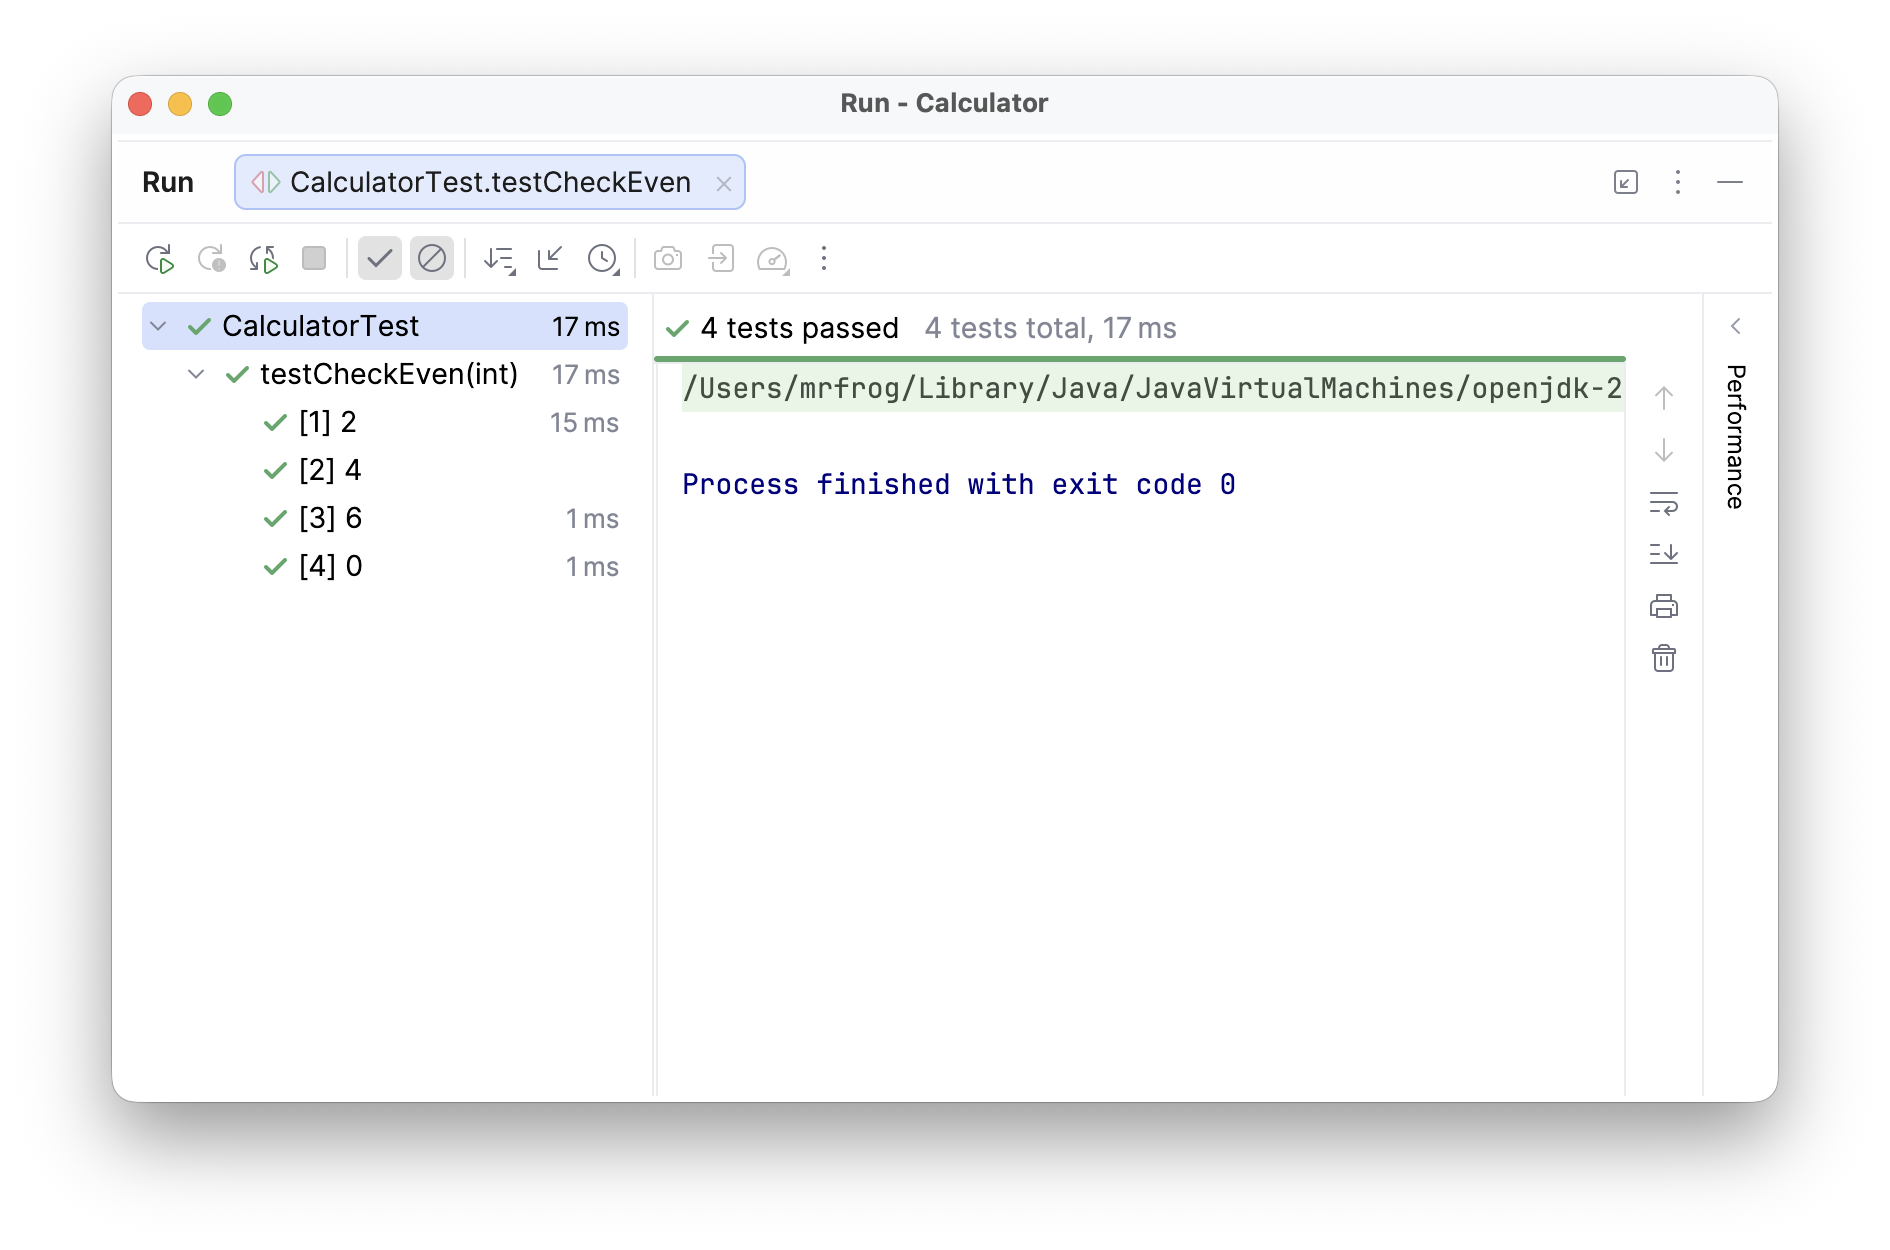
\includegraphics[width=0.95\textwidth]{01 - valuesourcetest.png}
    \caption{Hasil eksekusi parameterized test menggunakan ValueSource}
\end{figure}

\subsection{Pengujian Method \texttt{tambah} dengan \texttt{@CsvSource}}

Pengujian ini menggunakan tiga parameter sekaligus dalam format CSV yaitu nilai \texttt{a}, \texttt{b}, dan nilai \textit{expected}. Setiap baris data CSV akan dieksekusi sebagai satu skenario pengujian.

\begin{lstlisting}[style=commonstyle,language=Java,caption={Parameterized test CsvSource untuk method tambah}]
@ParameterizedTest
@CsvSource({"4,4,8", "100,100,200", "8,9,17"})
void testTambah(int a, int b, int expected) {
    Calculator cal = new Calculator(a,b);
    int actual = cal.tambah();
    assertEquals(expected, actual);
}
\end{lstlisting}

\begin{figure}[H]
    \centering
    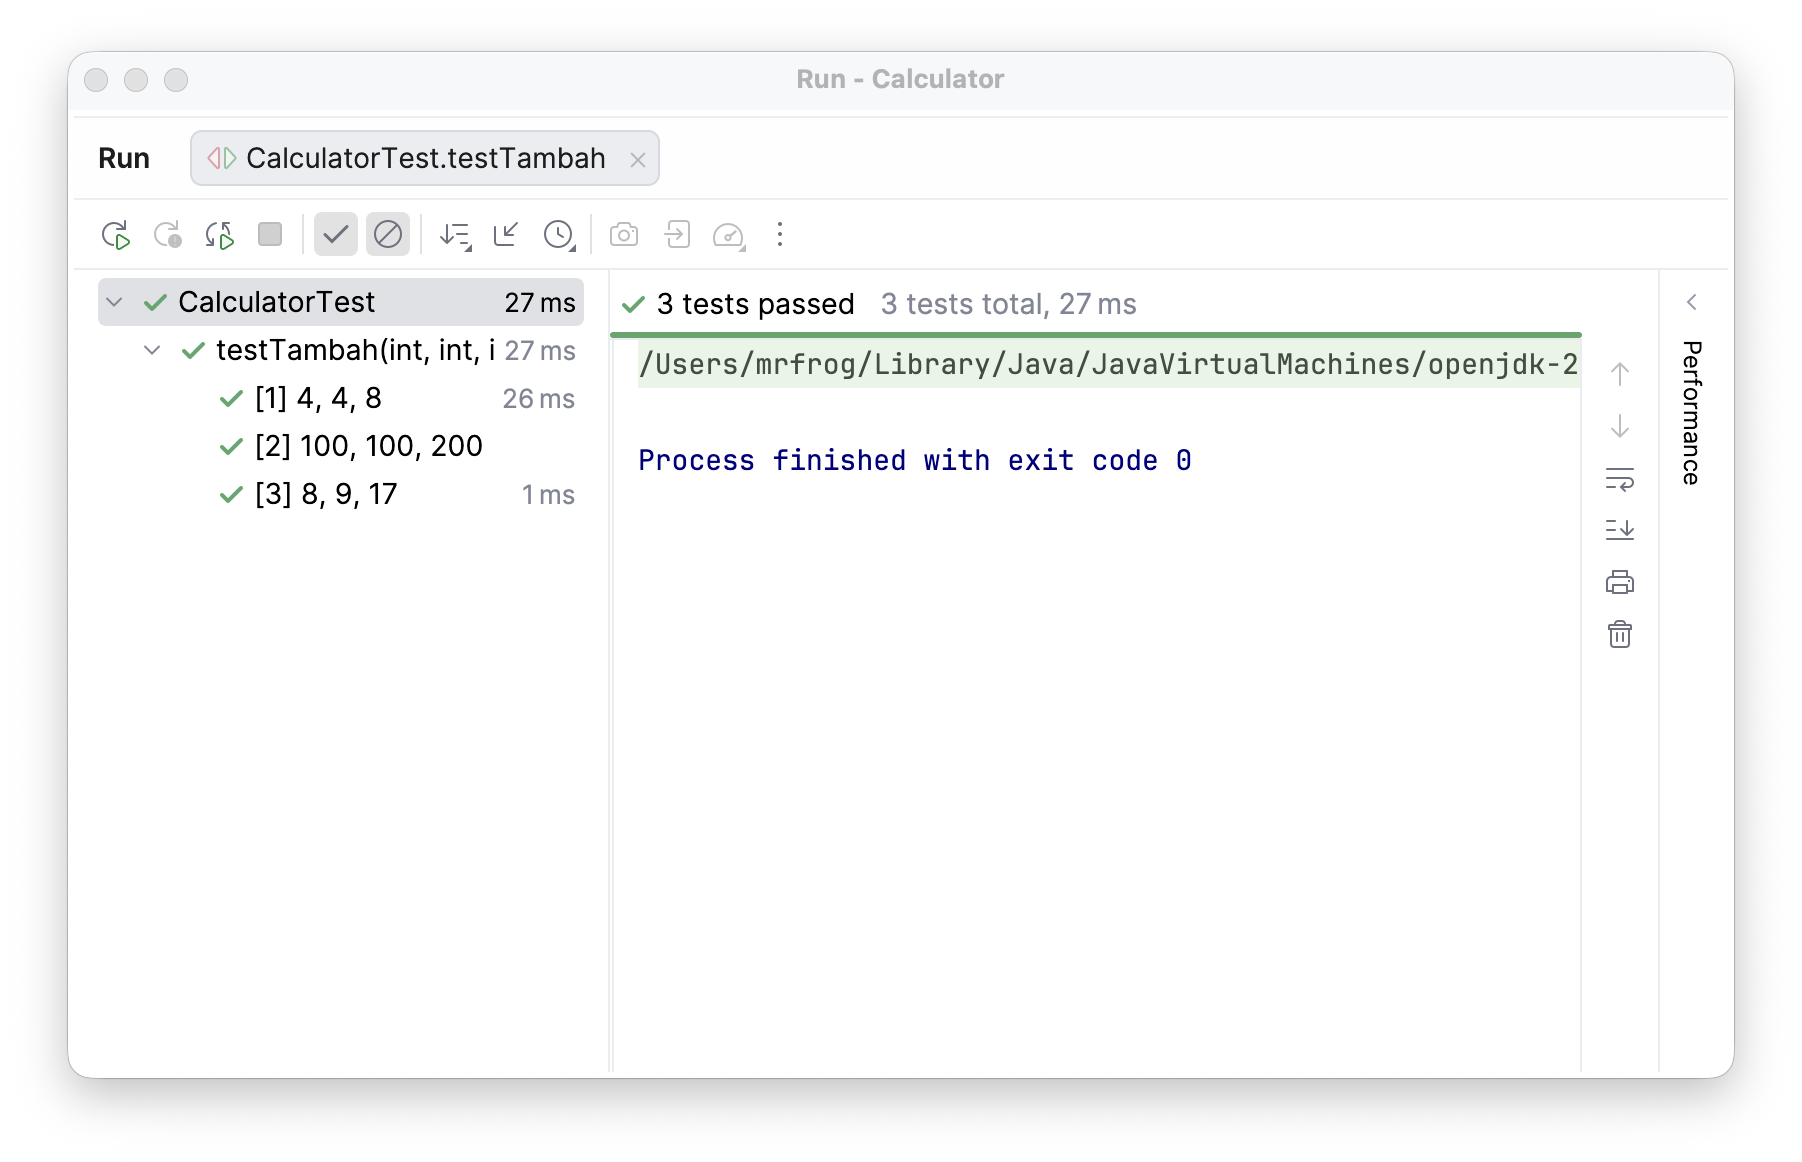
\includegraphics[width=0.95\textwidth]{02 - csvsourcetest.png}
    \caption{Hasil eksekusi parameterized test menggunakan CsvSource}
\end{figure}

\subsection{Pengujian Method \texttt{kurang} dengan \texttt{@MethodSource}}

Untuk \texttt{@MethodSource}, data parameter disediakan dari method terpisah bernama \texttt{data()}. Method ini mengembalikan \textit{stream} berisi kombinasi argument pengujian.

\begin{lstlisting}[style=commonstyle,language=Java,caption={Penyedia data dan test MethodSource untuk method kurang}]
private static Stream<Arguments> data() {
    return Stream.of(
        Arguments.of("2","5","-3"),
        Arguments.of("1","5","-4"),
        Arguments.of("5","8","-3")
    );
}

@ParameterizedTest
@MethodSource("data")
void testKurang(int a, int b, int expected) {
    Calculator cal = new Calculator(a,b);
    int actual = cal.kurang();
    assertEquals(expected, actual);
}
\end{lstlisting}

\begin{figure}[H]
    \centering
    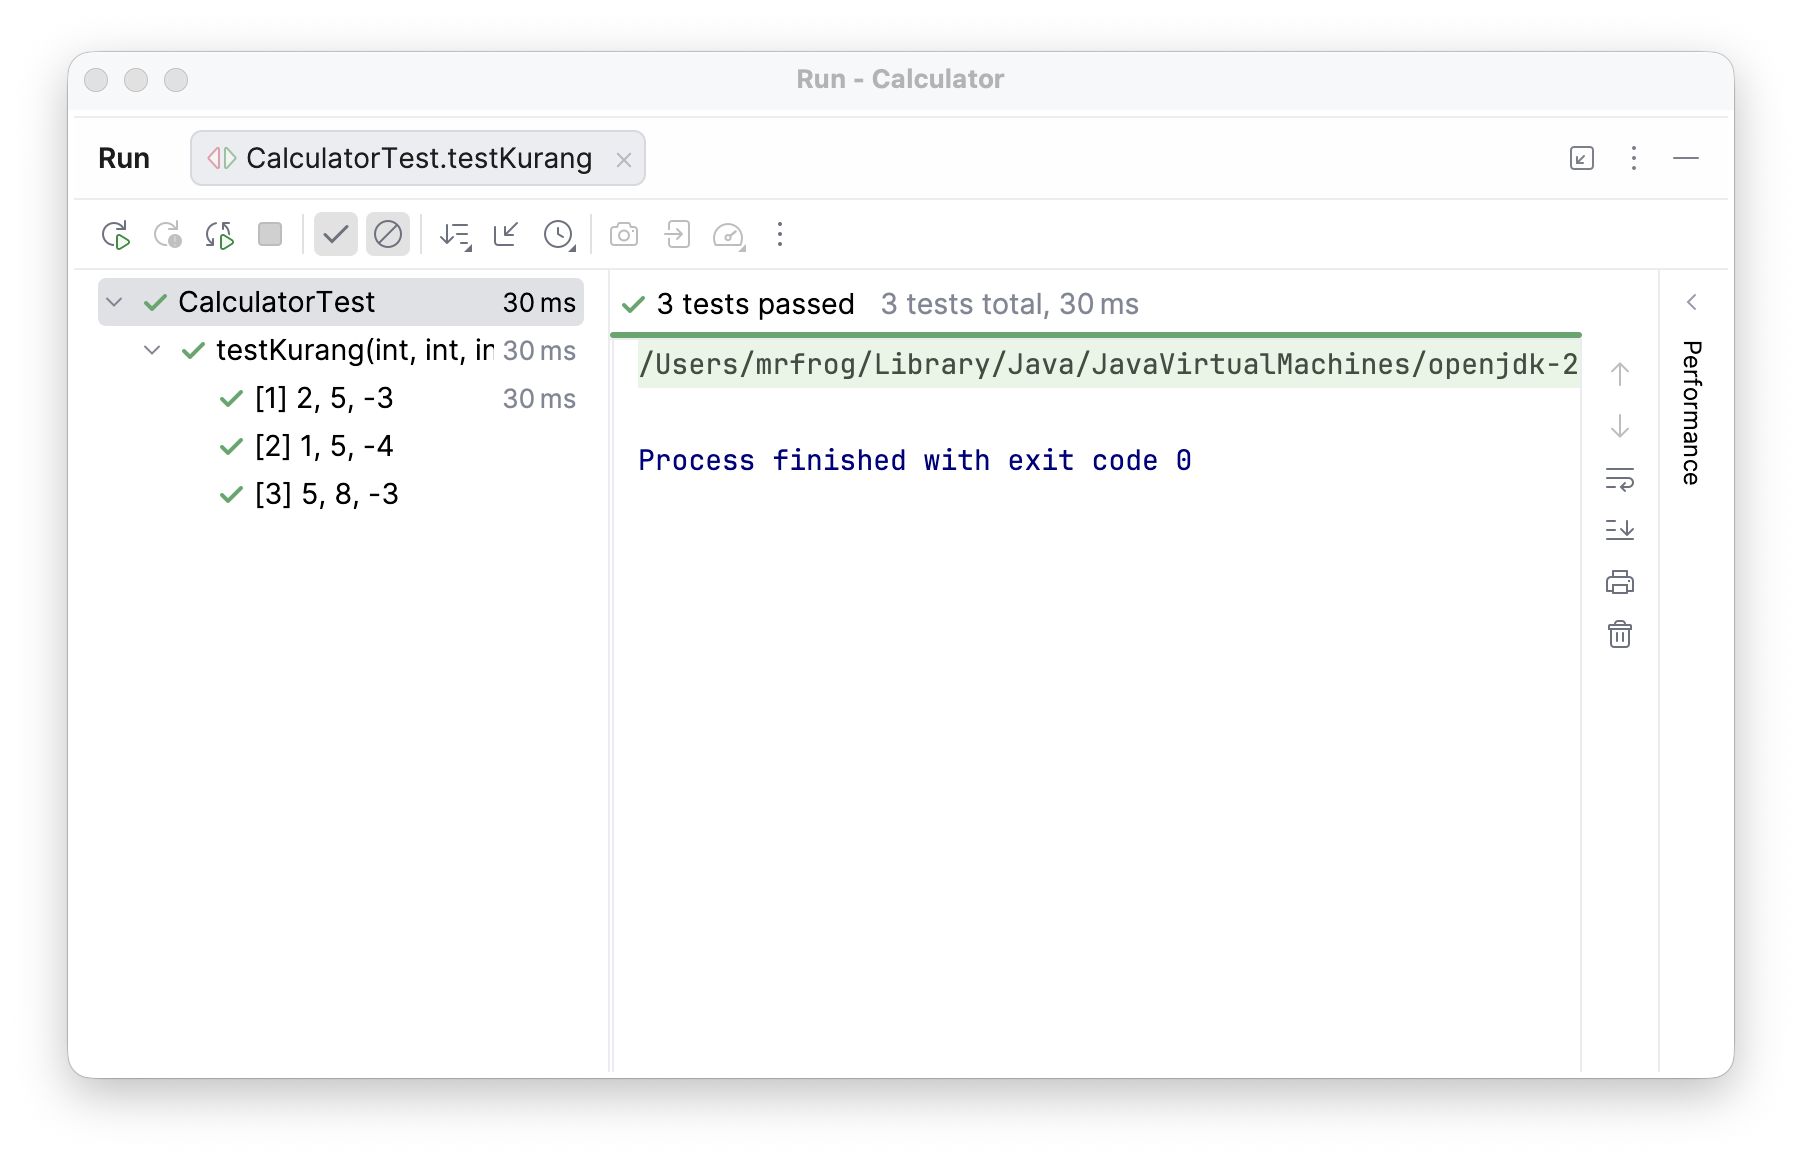
\includegraphics[width=0.95\textwidth]{03 - methodsourcetest.png}
    \caption{Hasil eksekusi parameterized test menggunakan MethodSource}
\end{figure}

\section{Tugas dan Analisis Praktikum}

\subsection{Validasi Nominal Cash dengan Single-value Parameter}

Pada studi kasus \textit{Wallet}, validasi nominal dilakukan melalui method \texttt{validBalance(int amount)}. Method mengembalikan \texttt{true} untuk nilai tidak negatif, dan \texttt{false} untuk nilai negatif. Pengujian dilakukan menggunakan \texttt{@ValueSource} untuk data valid dan tidak valid.

\begin{lstlisting}[style=commonstyle,language=Java,caption={Method validBalance dan pengujiannya dengan ValueSource}]
public boolean validBalance(int amount) {
    if (amount < 0) {
        return false;
    }
    return true;
}

@ParameterizedTest
@ValueSource(ints = {1000, 5000, 0})
void testBalancePositive(int amount) {
    Wallet wallet = new Wallet();
    assertTrue(wallet.validBalance(amount));
}

@ParameterizedTest
@ValueSource(ints = {-1000, -5000})
void testBalanceNegative(int amount) {
    Wallet wallet = new Wallet();
    assertFalse(wallet.validBalance(amount));
}
\end{lstlisting}

\begin{figure}[H]
    \centering
    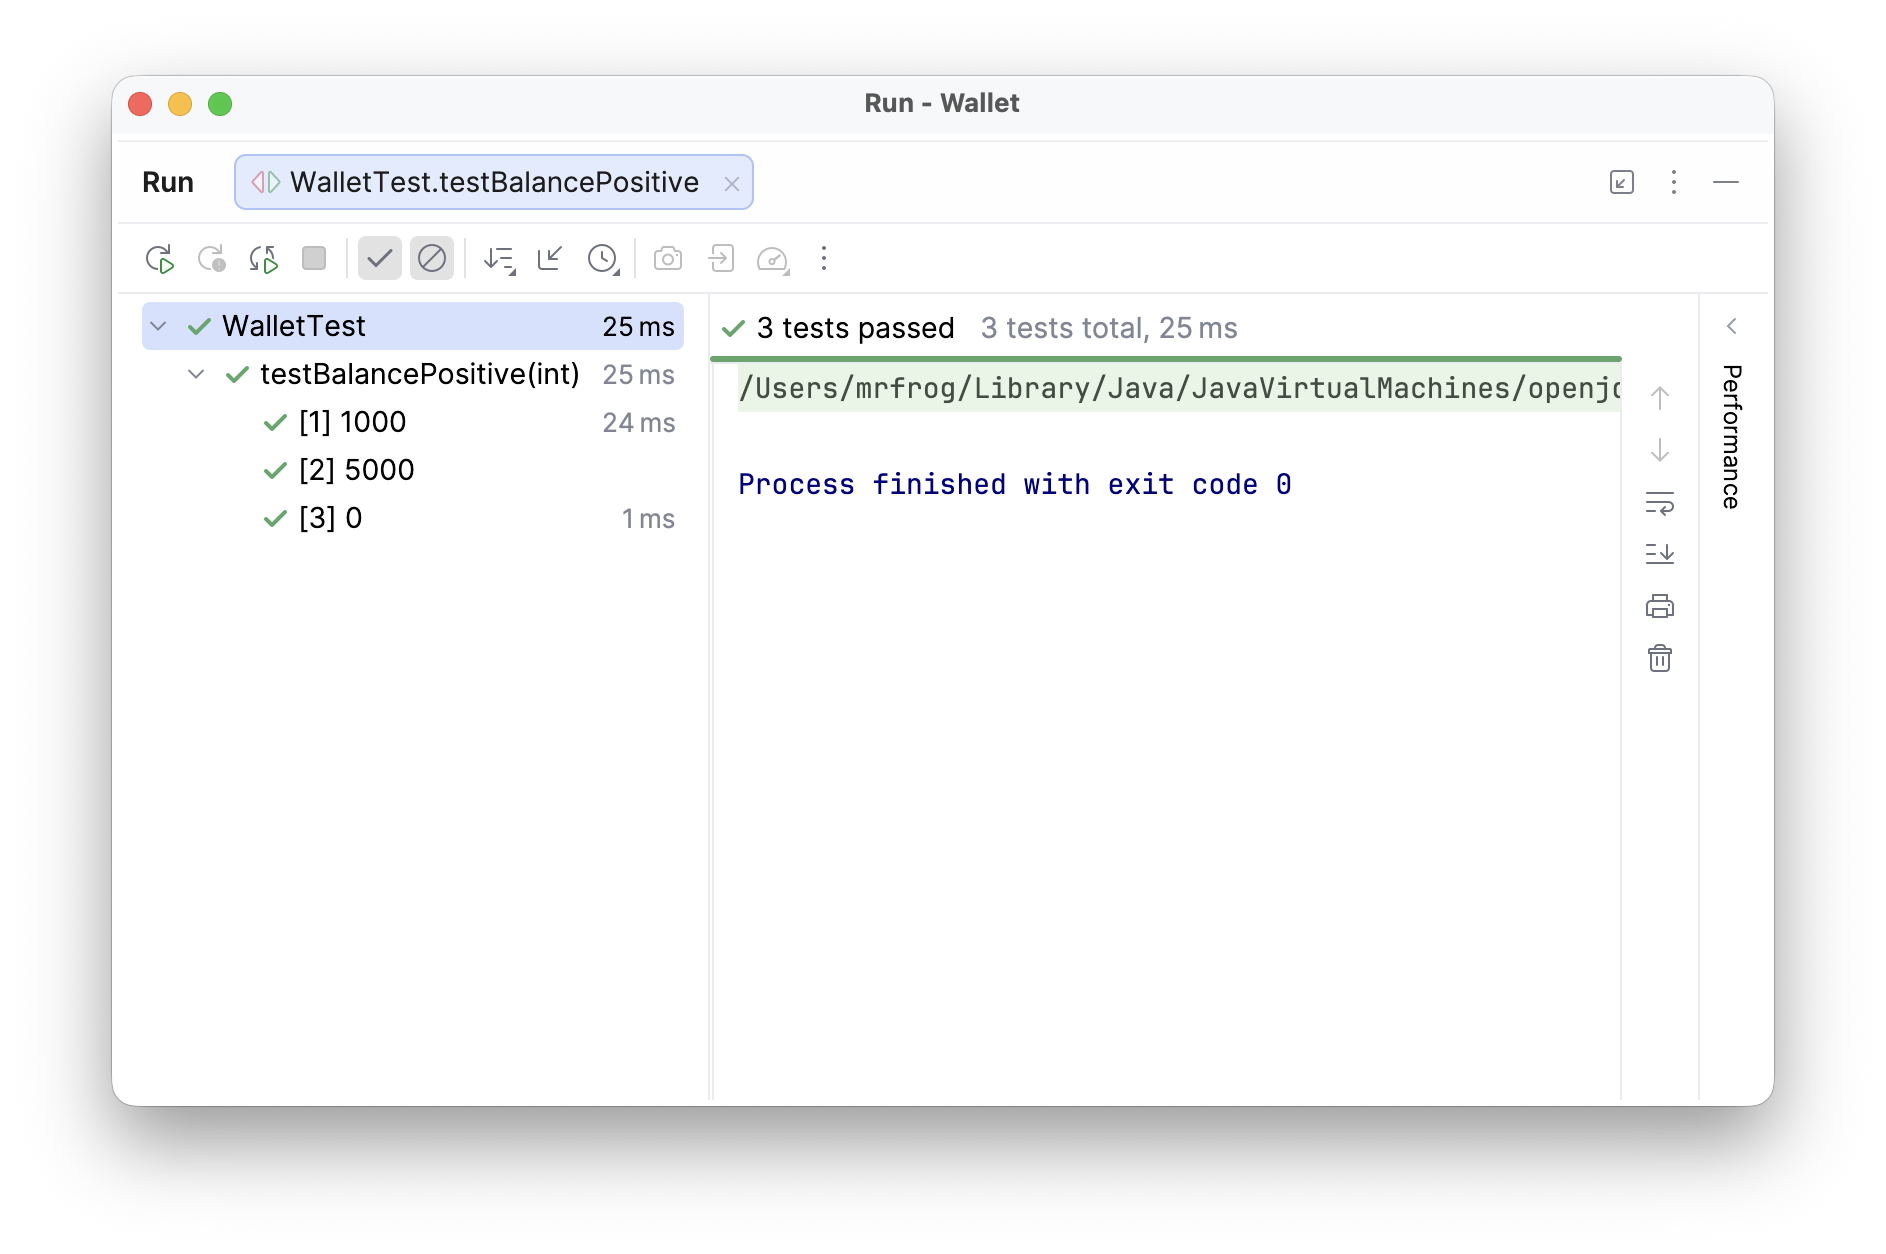
\includegraphics[width=0.95\textwidth]{04 - tugas balancepositive.png}
    \caption{Hasil pengujian nominal valid (balance positive)}
\end{figure}

\begin{figure}[H]
    \centering
    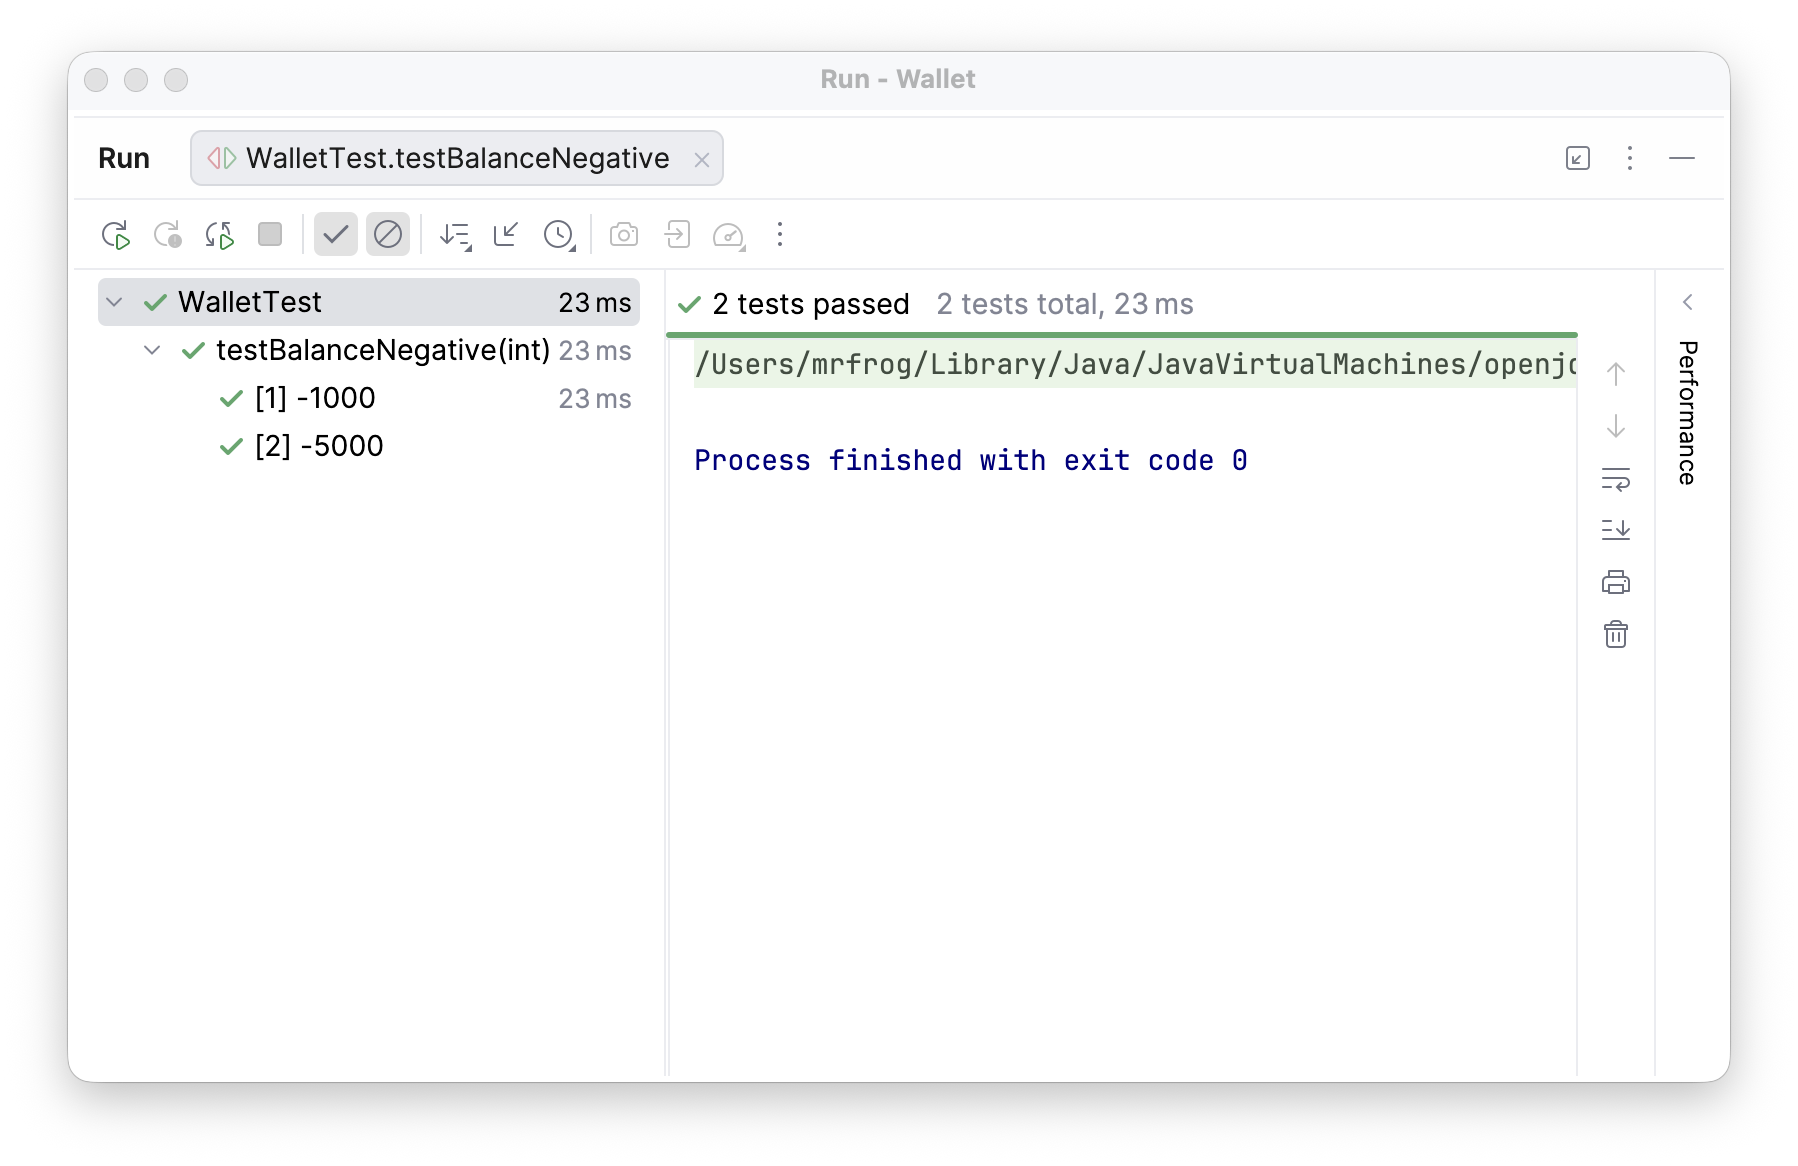
\includegraphics[width=0.95\textwidth]{04 - tugas abalancenegative.png}
    \caption{Hasil pengujian nominal tidak valid (balance negative)}
\end{figure}

\subsection{Pengujian Transaksi Withdraw untuk Data Valid dan Invalid}

Method \texttt{withdraw(int amount)} memiliki validasi khusus: nilai negatif dan nol akan melempar \texttt{IllegalArgumentException}, sedangkan nilai melebihi saldo akan melempar \texttt{InsufficientFundsException}. Skenario valid dan invalid diuji secara parameterized.

\begin{lstlisting}[style=commonstyle,language=Java,caption={Implementasi withdraw pada class Wallet}]
public boolean withdraw(int amount) {
    if (amount < 0) {
        throw new IllegalArgumentException("Amount cannot be negative");
    }
    if (amount > totalMoney) {
        throw new InsufficientFundsException("Amount cannot be greater than total money");
    }
    if (amount == 0) {
        throw new IllegalArgumentException("Amount cannot be zero");
    }
    totalMoney -= amount;
    return false;
}
\end{lstlisting}

\begin{lstlisting}[style=commonstyle,language=Java,caption={Parameterized test transaksi valid dan invalid}]
@ParameterizedTest
@CsvSource({"10000,5000,5000", "20000,5000,15000", "10000,9000,1000"})
void testTransaction(int deposit, int withdraw, int expected) {
    wallet.deposit(deposit);
    wallet.withdraw(withdraw);
    assertEquals(expected, wallet.getTotalMoney());
}

@ParameterizedTest
@CsvSource({
    "10000,15000,InsufficientFundsException",
    "10000,0,IllegalArgumentException",
    "10000,-1000,IllegalArgumentException",
    "0,1000,InsufficientFundsException"
})
void testTransactionInvalid(int deposit, int withdraw, String exceptionType) {
    if (deposit > 0) {
        wallet.deposit(deposit);
    }

    if (exceptionType.equals("InsufficientFundsException")) {
        assertThrows(InsufficientFundsException.class, () -> wallet.withdraw(withdraw));
    } else {
        assertThrows(IllegalArgumentException.class, () -> wallet.withdraw(withdraw));
    }
}
\end{lstlisting}

\begin{figure}[H]
    \centering
    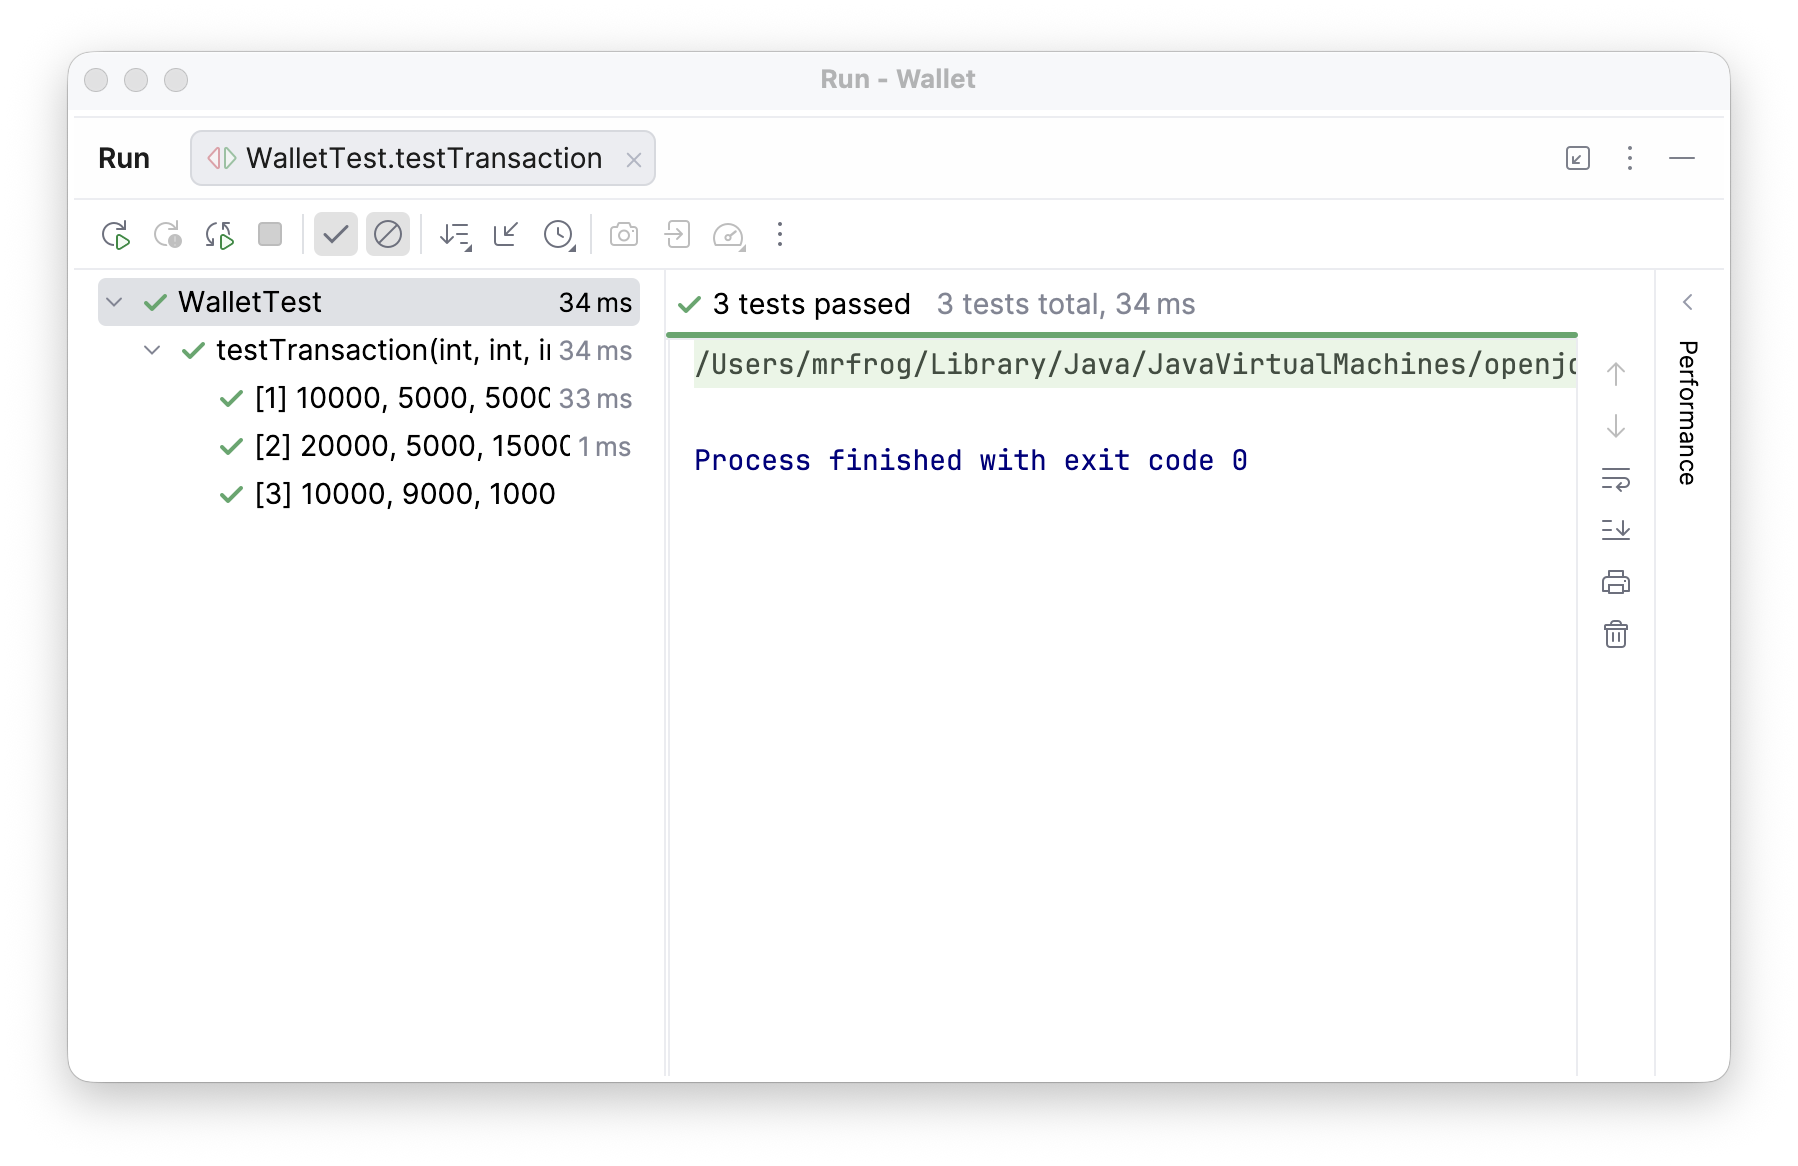
\includegraphics[width=0.95\textwidth]{05 - tugas testtransaction.png}
    \caption{Hasil pengujian transaksi valid}
\end{figure}

\begin{figure}[H]
    \centering
    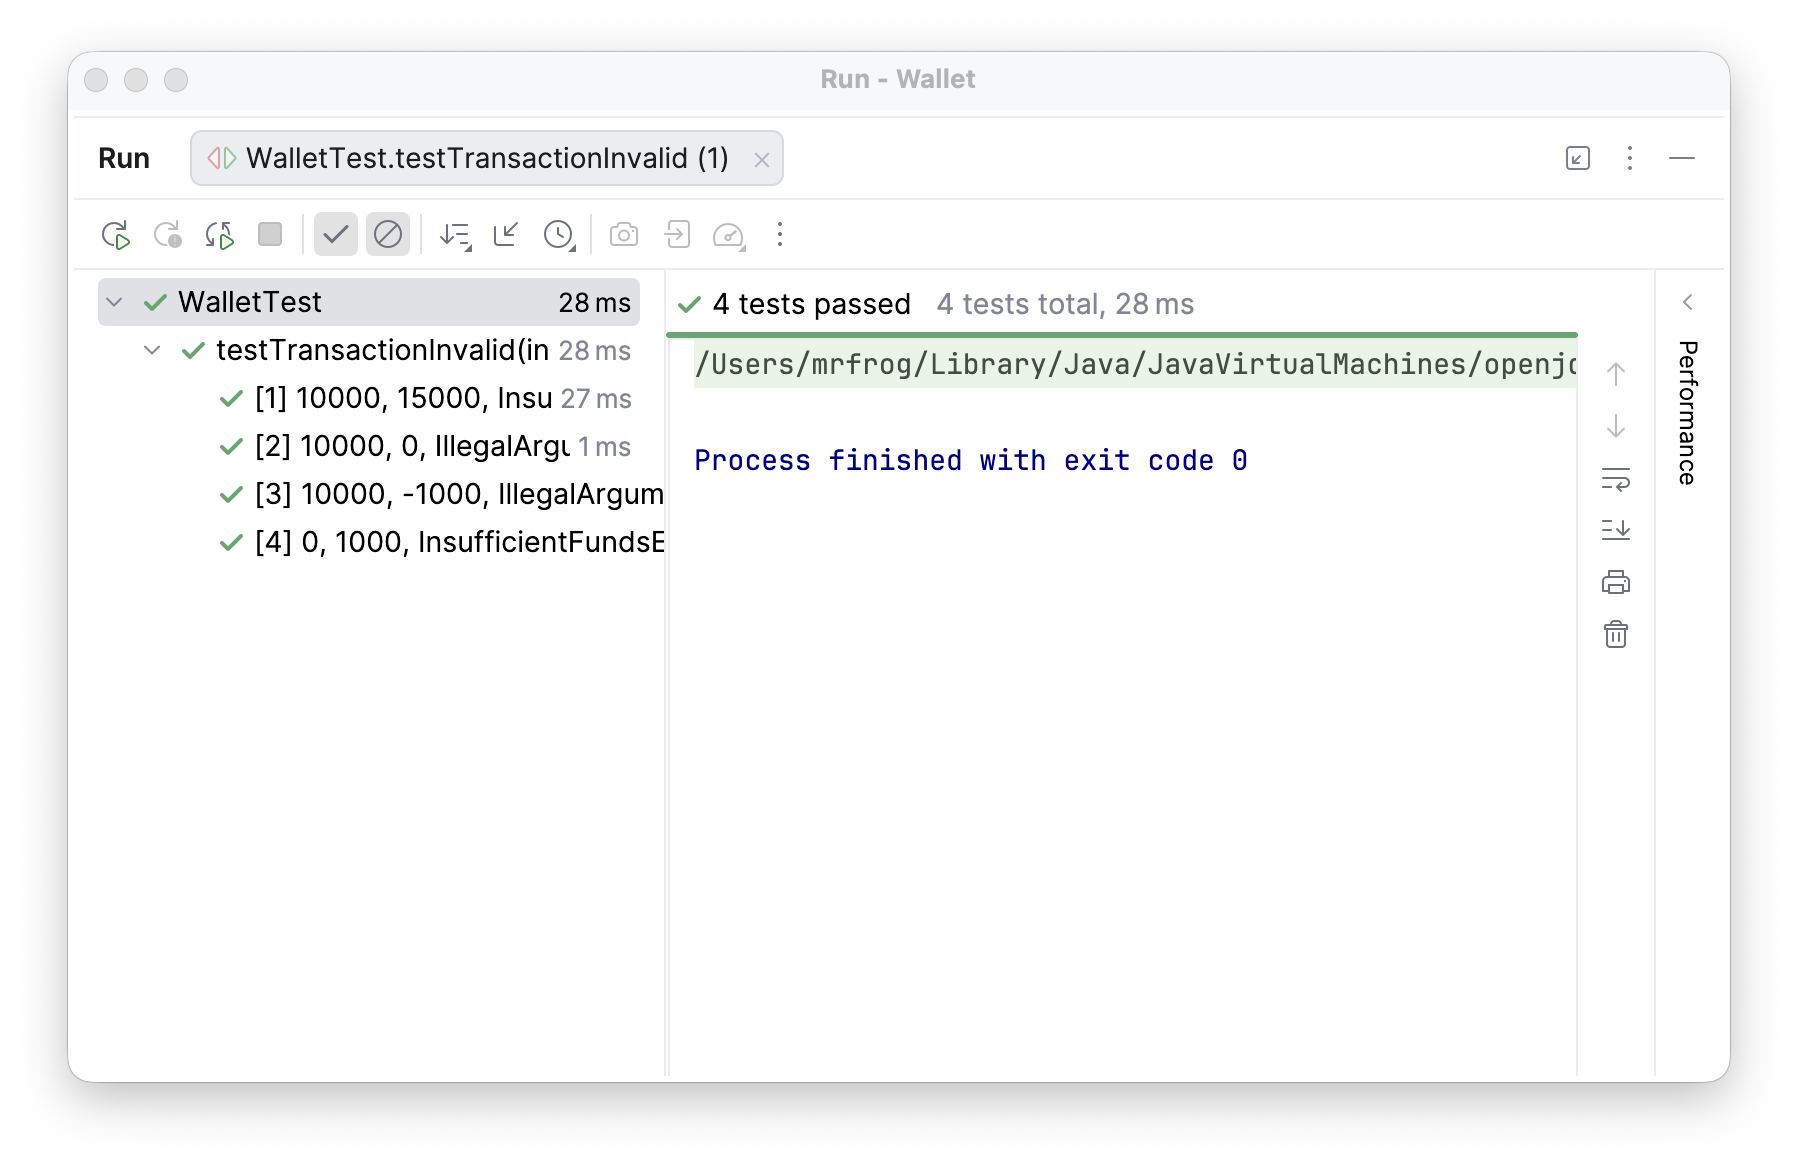
\includegraphics[width=0.95\textwidth]{06 - tugas testinvalidtransaction.png}
    \caption{Hasil pengujian transaksi invalid dengan assertion exception}
\end{figure}

\subsection{Implementasi Owner sebagai Object dan Pengujian MethodSource}

Sesuai ketentuan tugas, atribut \textit{owner} tidak lagi berupa \textit{string}, melainkan object dari class \texttt{Owner} yang memiliki \texttt{id}, \texttt{name}, dan \texttt{email}. Pengujian \texttt{setOwner(Owner owner)} dilakukan menggunakan \texttt{@MethodSource} dengan \textit{argument provider} object.

\begin{lstlisting}[style=commonstyle,language=Java,caption={Class Owner dan pengujian setOwner dengan MethodSource}]
public class Owner {
    private final String id;
    private final String name;
    private final String email;

    public Owner(String id, String name, String email) {
        this.id = id;
        this.name = name;
        this.email = email;
    }
}

private static Stream<Arguments> ownerProvider() {
    return Stream.of(
        Arguments.of(new Owner("1", "Budi", "budi@mail.com")),
        Arguments.of(new Owner("2", "Andi", "andi@mail.com")),
        Arguments.of(new Owner("3", "Sinta", "sinta@mail.com"))
    );
}

@ParameterizedTest
@MethodSource("ownerProvider")
void testSetOwner(Owner owner) {
    Wallet wallet = new Wallet();
    wallet.setOwner(owner);
    assertEquals(owner, wallet.getOwner());
}
\end{lstlisting}

\begin{figure}[H]
    \centering
    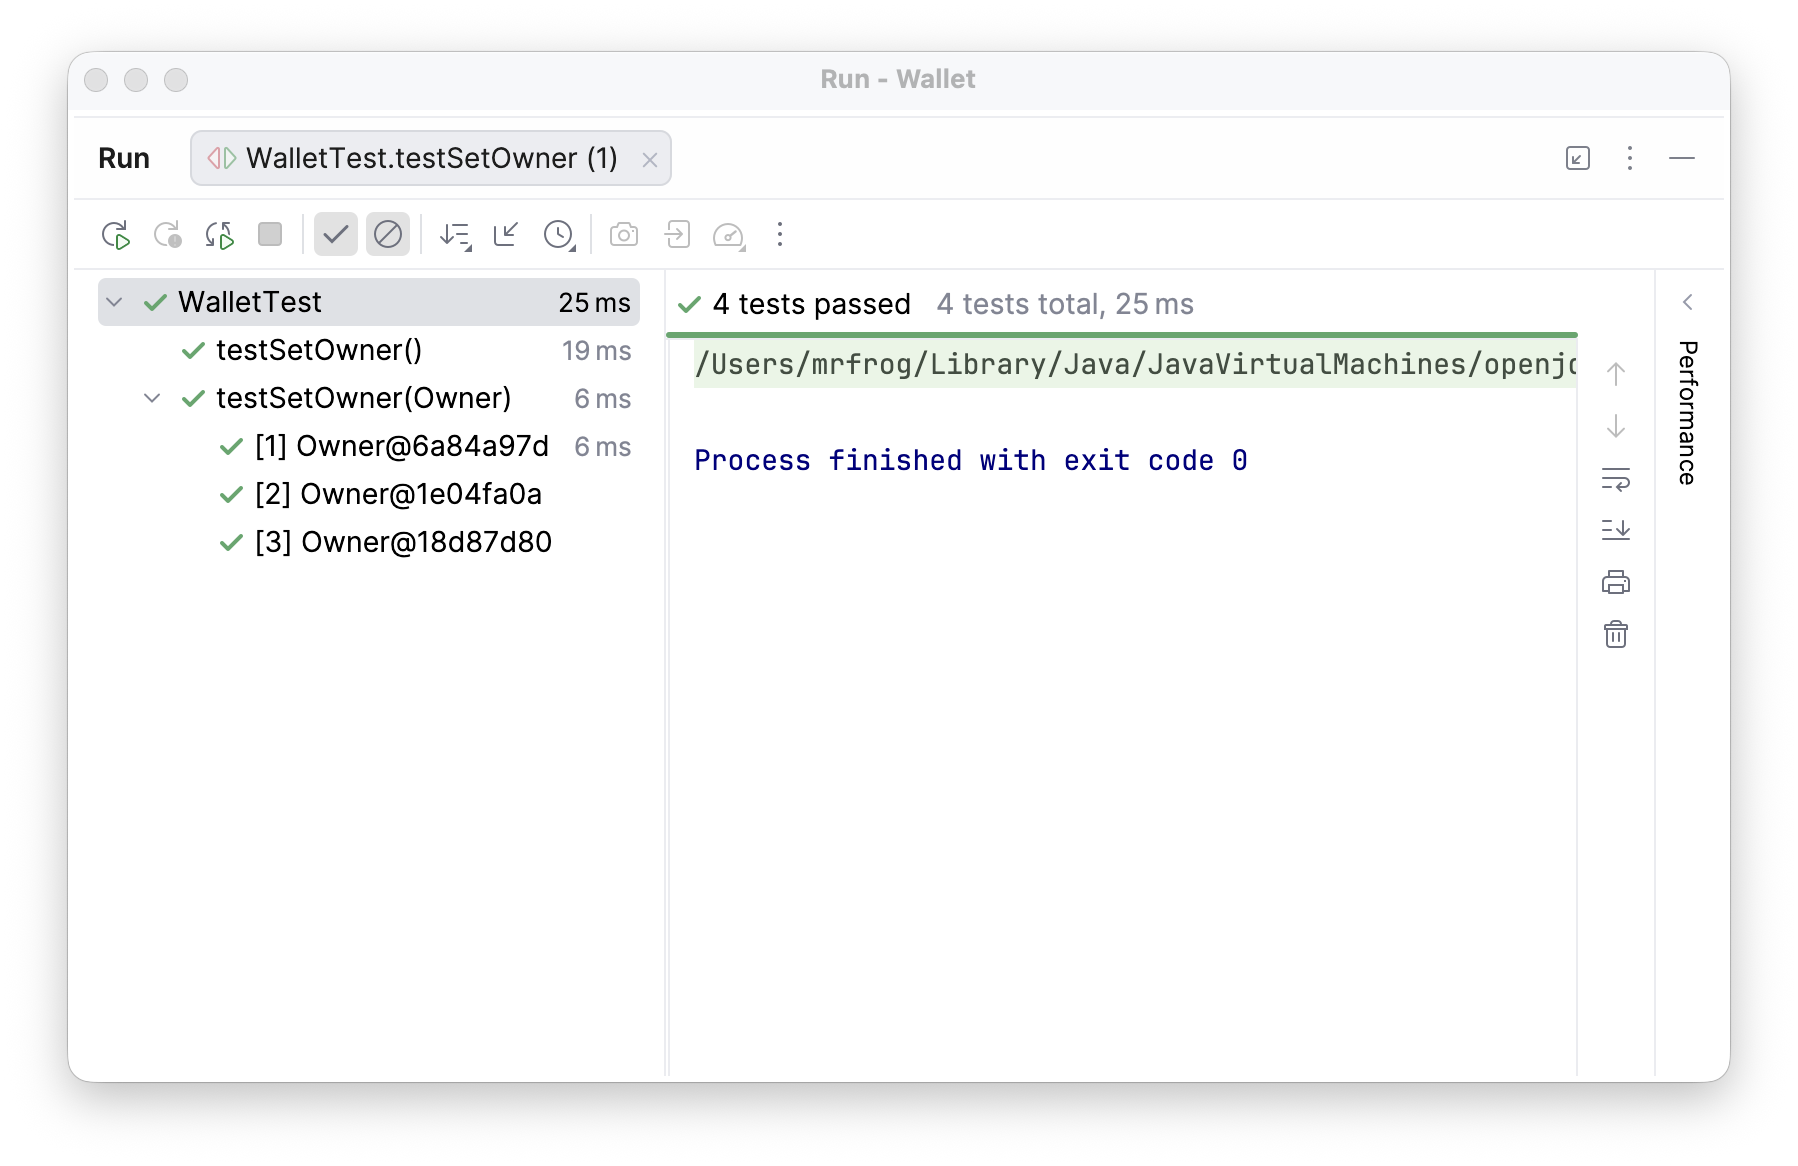
\includegraphics[width=0.95\textwidth]{07 - tugas ownertest.png}
    \caption{Hasil pengujian setOwner dengan MethodSource}
\end{figure}

\clearpage


\chapter{Resource}
Repository source code praktikum ini dapat diakses melalui GitHub berikut:

\begin{center}
    \url{https://github.com/januarsyah901/PPPL/tree/822cf2bb606fc8fd108707b2a7ef142aff78af1e/Pertemuan\%203}
\end{center}

\clearpage
\chapter{Kesimpulan}
Berdasarkan praktikum yang telah dilakukan, dapat disimpulkan bahwa \textit{parameterized test} pada JUnit 5 mempermudah pengujian banyak skenario dalam satu method uji. Penggunaan \texttt{@ValueSource}, \texttt{@CsvSource}, dan \texttt{@MethodSource} berhasil diterapkan pada studi kasus \textit{Calculator} dan \textit{Wallet}. Implementasi pengujian untuk kasus valid dan invalid, termasuk pengujian exception, membantu memastikan perilaku sistem lebih konsisten. Selain itu, perubahan \textit{owner} menjadi object class \texttt{Owner} meningkatkan struktur data dan fleksibilitas pengembangan lanjutan.

\clearpage
\end{document}
